\documentclass[12pt, a4paper, oneside]{ctexart}
\usepackage{amsmath,extarrows, amsthm, amssymb, bm, graphicx, hyperref, geometry, mathrsfs,color}
\usepackage{xcolor}
\usepackage{listings}
\usepackage{multicol}

\lstdefinestyle{lfonts}{
  basicstyle   = \footnotesize\ttfamily,
  stringstyle  = \color{purple},
  keywordstyle = \color{blue!60!black}\bfseries,
  commentstyle = \color{olive}\scshape,
}
\lstdefinestyle{lnumbers}{
  numbers     = left,
  numberstyle = \tiny,
  numbersep   = 1em,
  firstnumber = 1,
  stepnumber  = 1,
}
\lstdefinestyle{llayout}{
  breaklines       = true,
  tabsize          = 2,
  columns          = flexible,
}
\lstdefinestyle{lgeometry}{
  xleftmargin      = 20pt,
  xrightmargin     = 0pt,
  frame            = tb,
  framesep         = \fboxsep,
  framexleftmargin = 20pt,
}
\lstdefinestyle{lgeneral}{
  style = lfonts,
  style = lnumbers,
  style = llayout,
  style = lgeometry,
}
\lstdefinestyle{python}{
    language = {Python},
    style    = lgeneral,
}

\title{\huge\textbf{科学计算项目作业一}}
\author{罗俊勋\\学号:3210101613}
\date{\today}
\linespread{2}%行间距
\geometry{left=2cm,right=2cm,top=2cm,bottom=2cm}%设置页面
\CTEXsetup[format={\Large\bfseries}]{section}%section左对齐

%定义环境
\newenvironment{Def}[1][def-name]{\par\noindent{\textit{(#1):}\small}}{\\\par}
\newenvironment{theorem}[1][Theorem-name]{\par\noindent \textbf{Theorem #1:}\textit}{\\\par}
\newenvironment{corollary}[1][corollary-name]{\par\noindent \textbf{Corollary #1:}\textit}{\\\par\vspace*{15pt}}
\newenvironment{lemma}[1][lemma-name]{\par\noindent \textbf{Lemma #1:}\textbf}{\\\par}
\renewenvironment{proof}{\par\noindent{\textit{Proof:}\small}}{\\\par}
\newenvironment{example}[1][example-name]{\par{\textbf{Example:}}}{\\\par}
\newenvironment{say}{\center{\textit{summary:}}}{\\\par}
\newenvironment{note}[1][note-name]{\par\textit{#1:}}{\\\par}


\begin{document}
\maketitle

\section*{问题}
设你学号的最后一位是$z$,取$n = \max (2z,10).$\\
设函数$f(x)=\frac{1}{1+25x^2},x\in {[-1,1]}$.利用下列条件做插值逼近,并与函数$f(x)$的图像进行比较.\\

(a):用等距节点$x_i=-1+\frac{2i}{n},i=1,2,\cdots,n$.试建立$n$次$Lagrange$插值多项式和$Newton$插值多项式,绘出插值多项式的图像\\

(b):用节点$x_i=\cos{\frac{2i+1}{42}\pi},i = 0,1,2,\cdots ,20,$绘出20次$Lagrange$插值多项式的图像;\\

(c):用等距节点$x_i=-1+\frac{2}{10}i,i=0,1,2,\cdots,10,$绘出它的分段线性插值函数\\

(d):用等距节点$x_i=-1+\frac{2}{10}i,i=0,1,2,\cdots,10,$绘出它的分段三次$Hermite$插值函数的图像

\pagebreak
\section*{公式和算法}

{\color{red}{$Lagrange$插值原理:}}\\
{{$f(x)$是需要插值的函数;$(x_0,y_0),(x_1,y_1),\cdots,(x_n,y_n)$是$n+1$个插值节点};
\Def[计算方法]{令$\phi(x)=y_0l_0(x)+y_1l_1(x)+\cdots+y_nl_n(x)$
\center{
    若n次多项式$l_j(x);(j=0,1,2\cdots,n)$在n+1个节点$x_0<x_1<\ldots<x_n$上满足:\\
    $l_k\left(x_j\right)=\left\{\begin{array}{ll}1, & j=k \\ 0, & j\neq k\end{array},(j, k=0,1, \ldots, n)\right.$
    则称这n+1个n次多项式为节点$x_0<x_1<\ldots<x_n$上的n次插值基函数.\\
    lagrange:$l_k(x)=\prod\limits_{i=0,i\neq k}^n\frac{x-x_i}{x_k-x_i}=\frac{\left(x-x_0\right) \ldots\left(x-x_{k-1}\right)\left(x-x_{k+1}\right) \ldots\left(x-x_n\right)}{\left(x_k-x_0\right) \ldots\left(x_k-x_{k-1}\right)\left(x_k-x_{k+1}\right) \ldots\left(x_k-x_n\right)}$\\
    由此可得:$L_n(x)=\sum\limits_{k=0}^n y_k l_k(x)$称为lagrange插值函数}}
}
\vspace*{10pt}

{\color{red}{$Newton$插值原理:}}\\
{{$f(x)$是需要插值的函数;$(x_0,y_0),(x_1,y_1),\cdots,(x_n,y_n)$是$n+1$个插值节点}};
\Def[计算方法]{令$N(x)=f_0+f[x_0,x_1](x-x_0)+\cdots+f[x_0,x_1,\cdots,x_n](x-x_0)\cdots(x-x_{n-1})$}\\
其中$f[x_i,x_{i+1},\cdots,x_j]=\frac{f[x_i,x_{i+1},\cdots,x_{j-1}]-f[x_{i+1},x_{i+1},\cdots,x_j]}{x_i-x_j};f[x_i]=f(x_i);i=0,1,\cdots,n$
\vspace*{10pt}

{\color{red}{$Piecewise-Linear$分段线性插值原理:}}\\
{{$f(x)$是需要插值的函数;$(x_0,y_0),(x_1,y_1),\cdots,(x_n,y_n)$是$n+1$个插值节点}};
\Def[计算方法]{在每一区间$[x_i,x_{i+1}]$上使用线性插值得到基函数$\phi_i(x)=\frac{x-x_{i+1}}{x_i-x_{i+1}}y_i+\frac{x-x_{i}}{x_{i+1}-x_{i}}y_{i+1}$}.
再将所有的$\phi_i$并起来就是我们所需要的
\vspace*{10pt}

{\color{red}{$Piecewise-Hermite$分段$Hermite$插值原理:}}\\
设 $f \in C^1[a, b];(x_0,y_0,y'_0),(x_1,y_1,y'_1),\cdots,(x_n,y_n,y'_n)$是n+1个插值节点及其导数值.\\
如果函数 $\varphi(x)$ 满足:
(1) $\varphi \in C^1[a, b]$\\
(2) 满足揷值条件 $\varphi\left(x_k\right)=f\left(x_k\right),  \varphi^{\prime}\left(x_k\right)=f^{\prime}\left(x_k\right),k = 0,1,\cdots,n$\\
(3) 在每个小区间 $\left[x_k, x_{k+1}\right](k=0,1, \cdots, n-1)$ 上 $\varphi(x)$ 是一个三次多项式。 则称 $\varphi(x)$ 为 $f(x)$ 以 $a=x_0<x_1<\cdots<x_n=b$ 为节点的分段三次 Hermite 揷值多项式。
\pagebreak

\section*{程序}
必要的说明都在注释中
\begin{multicols}{2}
\begin{lstlisting}[style = python]
    import time
    import copy
    import numpy as np
    import sympy as sy
    import matplotlib.pyplot as plt
\end{lstlisting}

\begin{lstlisting}[style = python]
    #lagrange插值函数
    def Lagrange(x_list,y_list):
        n = len(x_list)
        result = Lagrange_basefunction_list(x_list,n)
        return sum([result[i]*y_list[i] for i in range(n)])
    
    def Lagrange_basefunction_list(x_list,n):    #基函数列
        result = []
        for i in range(n):
            result.append(Lagrange_basefunction(x_list,i))
        return result    
    def Lagrange_basefunction(x_list,i):    #基函数
        X_list = copy.deepcopy(x_list)
        x_i = X_list[i]
        del X_list[i]
        denominator = 1
        for item in X_list:
            denominator = denominator*(x_i-item)
        coefficients_1 = np.poly(X_list)        #计算分子函数的系数
        coefficients_2 = [value/denominator for value in coefficients_1]        #计算函数系数
        basefunc = np.poly1d(coefficients_2,r = False ,variable='x')        #基函数
        return basefunc
\end{lstlisting}

\begin{lstlisting}[style = python]
    #Newton插值函数
    def Newton(x_list,y_list):
        dim = len(x_list)
        mat = list([j for j in range(dim)] for i in range(dim))
        def f(i,j):        #定义差商函数
            if j==0:
                return y_list[i]
            else:
                return (f(i-1,j-1)-f(i,j-1))/(x_list[i-j]-x_list[i])
        for i in range(len(x_list)):        #计算矩阵
            for j in range(i+1):
                mat[i][j] = f(i,j)
        def N(k):        #定义返回x的多项式的函数
            func = 1
            if k != 0:
                func = np.poly1d(x_list[0:k],r = True ,variable = 'x')
            return func
        newton = 0
        for i in range(dim):
            newton += N(i)*mat[i][i]
        return newton
\end{lstlisting}

\begin{lstlisting}[style = python]
    #Hermite插值
    def Hermite(x_list,y_list,z_list):
        n = len(x_list)-1
        def h(x_list,i):
            f = 0
            x_i = x_list[i]
            for j in range(n+1):
                if j!=i:
                    f += 2*(np.poly1d([x_i],r=True,variable='x')/(x_list[j]-x_i))
            return (1+f)*Lagrange_basefunction(x_list,i)**2
        def H(x_list,i):
            return np.poly1d([x_list[i]],r=True,variable = 'x')*Lagrange_basefunction(x_list,i)**2
        hermite = 0
        for i in range(n+1):
            hermite += y_list[i]*h(x_list,i)+z_list[i]*H(x_list,i)
        return hermite
\end{lstlisting}

\begin{lstlisting}[style = python]
    #分段线性插值
    def Piecewise_Linear(x_list,y_list,x_0):
        n = len(x_list)-1
        def interval(x_list,x):        #定义区间函数
            for index in range(n):
                if x_list[index] <= x <=x_list[index+1]:
                    return index
        def phi(x_list,y_list,i):        #定义区间函数和函数字典
            f = y_list[i]*np.poly1d([x_list[i+1]],r=True,variable='x')/(x_list[i]-x_list[i+1])+\
            y_list[i+1]*np.poly1d([x_list[i]],r=True,variable='x')/(x_list[i+1]-x_list[i])
            return f
        phi_dict = {i:phi(x_list,y_list,i) for i in range(n)}
        index = interval(x_list,x_0)
        return phi_dict[index]
\end{lstlisting}


\begin{lstlisting}[style = python]
    #分段hermite插值
    def Piece_Hermite(x_list,y_list,z_list,x_0):
        n = len(x_list)-1
        def interval(x_list,x):   #定义区间函数
            for index in range(n):
                if x_list[index] <= x <=x_list[index+1]:
                    return index
        def piece(x_list,y_list,z_list,i):      #定义每一段上的插值函数
            x_lst = [x_list[i],x_list[i+1]]
            y_lst = [y_list[i],y_list[i+1]]
            z_lst = [z_list[i],z_list[i+1]]
            return Hermite(x_list=x_lst,y_list=y_lst,z_list=z_lst)
            #函数字典
        piece_hermit_dict = {i:piece(x_list,y_list,z_list,i) for i in range(n)}
        index = interval(x_list,x_0)
        return piece_hermit_dict[index]#返回区间函数
    
\end{lstlisting}

\begin{lstlisting}[style = python]
    #最终实现:这里只展示问题(b)的绘图,其余的情况是类似的
    n = max(10,int((input("请输入你的学号:\n"))[-1]))
    def f(x):
        return 1/(1+25*x**2) 
    def diff_f(x):
        return -50*x/(1+25*x**2)**2
    x_lst = np.arange(-1,1,0.001)
    y_lst = f(x_lst)
    def g(x): #定义插值节点函数
        import math
        return math.cos((2*x+1)*math.pi/42)
    x_list_2 = []
    y_list_2 = []
    for i in range(21):
        x_i = g(i)
        x_list_2.append(x_i)
        y_list_2.append(f(x_i))
    Lagrange_2 = Lagrange(x_list=x_list_2,y_list=y_list_2)
    x_2_L = np.arange(-1,1,0.01)
    y_2_L = Lagrange_2(x_2_L)
    plt.plot(x_lst,y_lst)
    plt.title('Lagrange Interpolation')
    plt.plot(x_2_L,y_2_L)
    plt.xlabel('x')
    plt.ylabel('lagrange_2')
    for i in range(21):
        plt.scatter(x_list_2[i],y_list_2[i])
    plt.show()
\end{lstlisting}
\end{multicols}  


\section*{数据结果}
运行以上程序生成五张图像,按顺序依次为(a)中$lagrange$插值图像,$Newton$插值图像;
(b)$Lagrange$插值图像;(c)分段线性插值图像;(d)分段三次$Hermite$插值图像\\
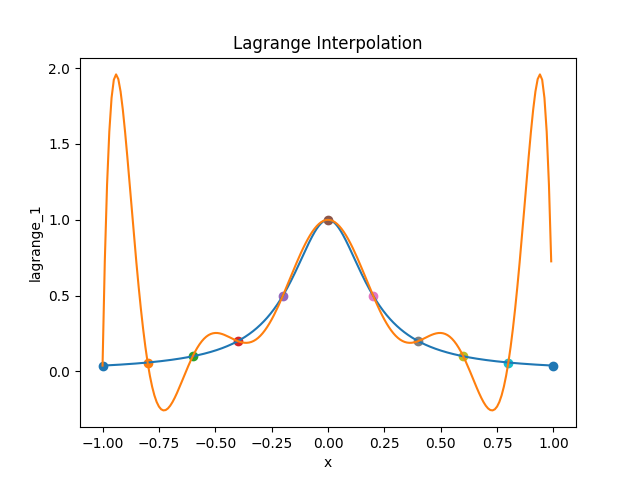
\includegraphics[scale=0.55]{Lagrange_1.png}
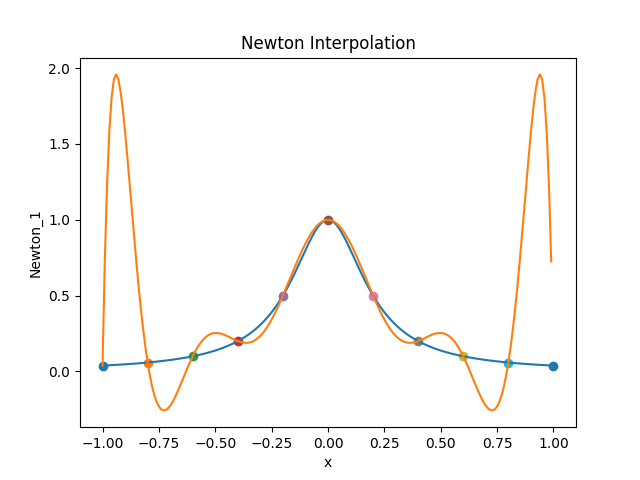
\includegraphics[scale=0.55]{Newton_1.png}
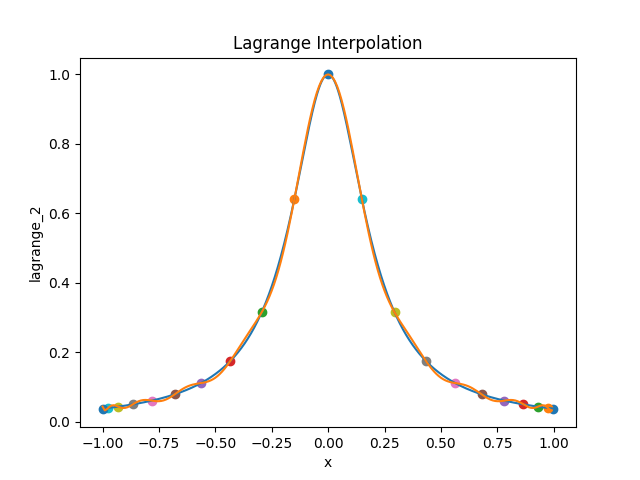
\includegraphics[scale=0.55]{Lagrange_2.png}
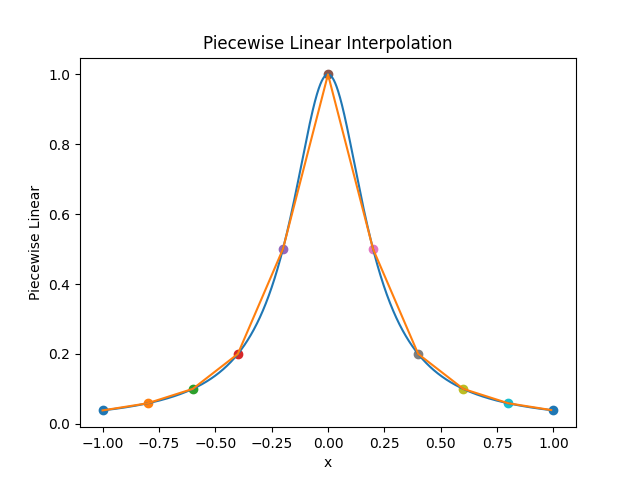
\includegraphics[scale=0.55]{Piecewise_Linear_3.png}
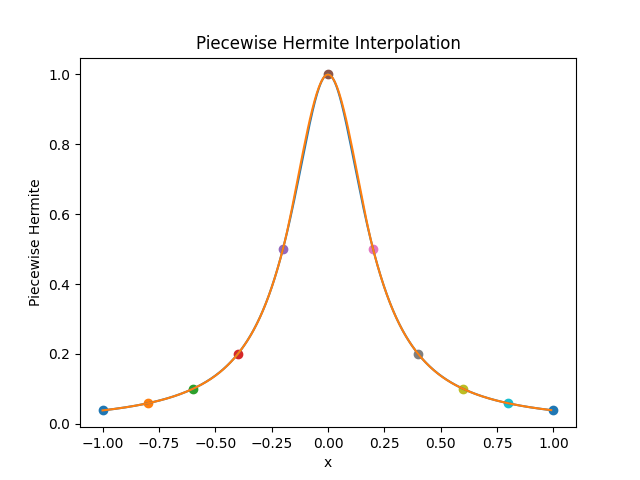
\includegraphics[scale=0.6]{Piecewise_Hermite_.4png.png}

\section*{结论}

1.从前两张图分钟可以看出$Lagrange$插值和$Newton$插值得到的函数是相同的,并且采用等距插值节点时
$Lagrange$插值和$Newton$插值在$0$附近的拟合效果很好,但是当$|x|>0.3$左右的时候,插值函数出现了剧烈的抖动,
精确度断崖式下降,当$x\to 0.9$的时候,误差更是达到了原函数值的四倍之多.\par

2.当插值节点更加密集分布在$0.3<|x|<1$中时,$Lagrange$插值函数的拟合效果比等距节点好的多,在0附近同样有较好的拟合效果,
当$|x|>0.3$时函数仅有微小的波动.\par

3.采用等距节点时,分段线性插值函数在0附近的拟合效果不及$x\to 1$时的效果,但是依旧没有很大的误差.整体来说拟合程度较好.
相对的缺点就是在节点处曲线不光滑.\par

4.分段$Hermite$插值的拟合效果是最好的,在$[-1,1]$上几乎与原函数重合.\par

总的来说,分段$Hermite$插值的拟合效果最好,但是在运行中可以发现其求解速度与其他方法有明显差距;
分段线性插值在函数变化不剧烈,节点较多时效果也很好;$Lagrange$插值和$Newton$插值的拟合效果受节点选取的影响很大,
适当的选择插值节点可以获得更精确的插值函数.

\end{document}